\section{GIÁ TRỊ LƯỢNG GIÁC CỦA GÓC LƯỢNG GIÁC}
\subsection{LÝ THUYẾT CẦN NHỚ}

\subsubsection{GÓC LƯỢNG GIÁC}

	\iconMT \indam{Góc lượng giác và số đo của góc lượng giác:} Trong mặt phẳng, cho hai tia $Ou$, $Ov$. Xét tia $Om$ cùng nằm trong mặt phẳng này. \\
	\indamm{Ghi nhớ 1:} Nếu tia $Om$ quay quanh điểm $O$, theo một chiều nhất định từ $Ou$ đến $Ov$, thì ta nói nó quét một góc lượng giác với tia đầu $Ou$, tia cuối $Ov$ và kí hiệu là $(\mathrm{O} u, \mathrm{O} v)$.
	\begin{center}		
	\begin{tikzpicture}[line width=1pt, >=Stealth,scale=.8]
		\def\bk{0.5}
		\def\dr{2.3}
		\draw (0,0)coordinate(O)node[below left=-1pt]{$O$} ;
		\draw (O) -- (0:\dr)node[pos=0.8, below]{$u$};
		\draw (O) --++(60:\dr)coordinate(M)node[left]{$v$};
		\draw [dashed,cyan] (O) --++(20:\dr)coordinate(M)node[above]{$m$};
		\foreach \a in {0.2}{
			\draw [->, red] ($(O)+(0:\bk+\a)$) arc (0:60:{\bk+\a} and {\bk+ \a})
			;
		}
		\draw [->,cyan] ($(O)!0.6!(M)$) arc (20:50:{0.5*\dr} and  {0.5*\dr})node[pos=0.5, above right=-1pt]{$+$} ;
	\end{tikzpicture}
	\begin{tikzpicture}[line width=1pt, >=Stealth,scale=.8]
		\def\bk{0.5}
		\def\dr{2.3}
		\draw (0,0)coordinate(O)node[below left=-2pt]{$O$} ;
		\foreach \a in {0.2}{
			\draw [->, red] ($(O)+(0:\bk+\a)$) arc (0:270:{\bk+\a} and {\bk+ \a})
			($(O)+(270:\bk+\a)$) arc (270:360:{\bk+\a+0.2} and {\bk +\a}) arc (360:415:{\bk+\a} and {\bk +\a})
			;
		}
		\draw (O) -- (0:\dr)node[pos=0.8, below]{$u$};
		\draw (O) -- (45:\dr)node[pos=0.8, below]{$v$};
		\draw [dashed,cyan] (O) --++(80:\dr)coordinate(M)node[above]{$m$};
		\draw [->,cyan] ($(O)!0.5!(M)$) arc (30:70:{0.7*\dr} and  {0.2*\dr})node[pos=0.5, above]{$+$} ;
	\end{tikzpicture}	
	\begin{tikzpicture}[line width=1pt, >=Stealth,scale=.8]
		\def\bk{0.5}
		\def\dr{2.3}
		\draw (0,0)coordinate(O)node[below left=-2pt]{$O$} ;
		\foreach \a in {0.2}{
			\draw [->, red] ($(O)+(0:\bk+\a)$) arc (0:-315:{\bk+\a} and {\bk+ \a})
			;
		}
		\draw (O) -- (0:\dr)node[pos=0.8, below]{$u$};
		\draw (O) -- (45:\dr)node[pos=0.8, below]{$v$};
		\draw [dashed,cyan] (O) --++(120:\dr)coordinate(M)node[above]{$m$};
		\draw [->,cyan] ($(O)!0.5!(M)$) arc (120:70:{0.7*\dr} and  {1*\dr})node[pos=0.5, above]{$-$} ;
	\end{tikzpicture}
	\end{center}

	\indamm{Ghi nhớ 2:}
		\begin{itemize}
			\item Khi tia $Om$ quay một góc $\alpha^\circ$, ta nói số đo của góc lượng giác $(Ou, Ov)$ bằng $\alpha^\circ$, kí hiệu $\text{sđ}(Ou, Ov)=\alpha^\circ$ hoặc $(Ou, Ov)=\alpha^\circ$.
			\item Mỗi góc lượng giác gốc $O$ được xác định bởi tia đầu $Ou$, tia cuối $Ov$ và số đo $\alpha^\circ$ của nó.
			\begin{center}
			\begin{tikzpicture}[line width=1pt, >=Stealth,scale=.8]
				\def\bk{0.5}
				\def\dr{2.3}
				\draw (0,0)coordinate(O)node[below left]{$O$} ;
				\foreach \a in {0.2}{
					\draw [->, red] ($(O)+(0:\bk+\a)$) arc (0:270:{\bk+\a} and {\bk+ \a})
					($(O)+(270:\bk+\a)$) arc (270:360:{\bk+\a +0.15} and {\bk +\a})
					;
				}
				\draw (O) -- (0:\dr)node[pos=0.8, below]{$u, v$};
				\draw [dashed,cyan] (O) --++(30:\dr)coordinate(M)node[above]{$m$};
				\draw [->,cyan] ($(O)!0.5!(M)$) arc (30:70:{0.5*\dr} and  {0.5*\dr})node[pos=0.5, above right=-1pt]{$+$} ;
				\node[below right] at (-1,-1) {\footnotesize$\text{sđ}(Ou, Ov)=360^\circ$};
			\end{tikzpicture} 
			\begin{tikzpicture}[line width=1pt, >=Stealth,scale=.8]
				\def\bk{0.5}
				\def\dr{2.1}
				\path
				(0:0) coordinate (O)
				(0:\dr) coordinate (A)
				(45:\dr) coordinate (B)
				;
				\draw pic["\tiny$45^\circ$",draw,angle eccentricity=1.8,angle radius=0.3cm]{angle=A--O--B};
				\draw (0,0)coordinate(O)node[below left=-2pt]{$O$} ;
				\foreach \a in {0.3}{
					\draw [->, red] ($(O)+(0:\bk+\a)$) arc (0:270:{\bk+\a} and {\bk+ \a})
					($(O)+(270:\bk+\a)$) arc (270:360:{\bk+\a+0.2} and {\bk +\a}) arc (360:415:{\bk+\a} and {\bk +\a})
					;
				}
				\draw (O) -- (0:\dr)node[pos=0.8, below]{$u$};
				\draw (O) -- (45:\dr)node[pos=0.8, below]{$v$};
				\draw [dashed,cyan] (O) --++(80:\dr)coordinate(M)node[above]{$m$};
				\draw [->,cyan] ($(O)!0.5!(M)$) arc (30:70:{0.7*\dr} and  {0.2*\dr})node[pos=0.5, above]{$+$} ;
				\node[below right] at (-1,-1) {\footnotesize$\text{sđ}(Ou, Ov)=405^\circ$};
			\end{tikzpicture}
			\begin{tikzpicture}[line width=1pt, >=Stealth,scale=.8]
				\def\bk{0.5}
				\def\dr{2.3}
				\draw (0,0)coordinate(O)node[above]{$O$} ;
				\foreach \a in {0.2}{
					\draw [ red] ($(O)+(0:\bk+\a)$) arc (0:-270:{\bk+\a} and {\bk+ \a})
					($(O)+(-270:\bk+\a)$) arc (-270:-360:{\bk+\a +0.15} and {\bk +\a})
					;
				}
				\foreach \a in {0.35}{
					\draw [->, red] ($(O)+(0:\bk+\a)$) arc (0:-90:{\bk+\a} and {\bk+ \a})
					($(O)+(-90:\bk+\a)$) arc (-90:-180:{\bk+\a} and {\bk +\a})
					;
				}
				\draw (O) -- (0:\dr)node[pos=0.8, below]{$u$};
				\draw [dashed,cyan] (O) --++(-30:\dr)coordinate(M)node[above]{$m$};
				\draw [->,cyan] ($(O)!0.5!(M)$) arc (-30:-70:{0.5*\dr} and  {0.5*\dr})node[pos=0.5, below right=-1pt]{$-$} ;
				\draw [red] (O)--++(180:\dr)node[below]{$v$};
				\node[below right] at (-1,-1.6) {\footnotesize$\text{sđ}(Ou, Ov)=-540^\circ$};
			\end{tikzpicture}			
			\end{center}
			\item Số đo của các góc lượng giác có cùng tia đầu $Ou$ và tia cuối $Ov$ sai khác nhau một bội nguyên của $360^{\circ}$ nên
			\boxmini{$\text{sđ}(Ou, Ov)=\alpha^{\circ}+k 360^{\circ}, \text{ với } k \in \mathbb{Z}$}
		\end{itemize}

	\iconMT \indam{Hệ thức Chasles:} Với ba tia $Ou$, $Ov$, $Ow$ bất kì, ta có
	\boxmini{$\text{sđ}(Ou,Ov)+\text{sđ}(Ov,Ow)=\text{sđ}(Ou, Ow)+k360^{\circ} \quad \text{với } k \in \mathbb{Z}.$}


\subsubsection{ĐƠN VỊ ĐO GÓC VÀ ĐỘ DÀI CUNG TRÒN}
\iconMT \indam{Đơn vị đo góc:}
	\begin{itemize}
		\item Đơn vị độ ($^\circ$): Chia đường tròn thành 360 cung tròn bằng nhau thì góc ở tâm chắn bởi cung đó sẽ có số đo là $1^\circ$.
		\item Đơn vị rađian (rad): Trên đường tròn, nếu một cung tròn có độ dài bằng bán kính thì ta nói cung đó có số đo là 1 rad. Khi đó, góc ở tâm chắn cung đó cũng có số đo 1 rad.
		\begin{note}
			Khi viết số đo một góc theo đơn vị rad, ta thường không viết chữ rad sau số đo. Chẳng hạn góc $\dfrac{\pi}{2}$ ta hiểu là góc $\dfrac{\pi}{2}$ rad.
		\end{note}
		\item Mối liên hệ giữa độ và rađian:
		\boxmini{$1^\circ=\dfrac{\pi}{180}\, \mathrm{rad} \quad \text{ và } \quad 1\, \mathrm{rad}=\left(\dfrac{180}{\pi}\right)^\circ$}
	\end{itemize}
\iconMT \indam{Độ dài cung tròn:} Một cung của đường tròn bán kính $R$ có số đo $\alpha$ rad thì sẽ có độ dài là \boxmini{$l=R\alpha=R\dfrac{a^\circ \pi}{180^\circ}$.}


\subsubsection{GIÁ TRỊ LƯỢNG GIÁC CỦA MỘT GÓC LƯỢNG GIÁC}
\iconMT \indam{Đường tròn lượng giác:} 
	\immini[thm]{
		\begin{itemize}
			\item Trong mặt phẳng tọa độ, đường tròn tâm $O$ bán kính 1, cùng với gốc $A(1;0)$ và chiều quay dương (như quy ước) gọi là \textit{đường tròn lượng giác}.
			\item Cho góc lượng giác số đo $\alpha$. Trên đường tròn lượng giác, tồn tại duy nhất điểm $M$ sao cho góc lượng giác $(OA,OM)$ bằng $\alpha$. Khi đó, $M$ gọi là \textit{điểm biểu diễn của góc có số đo }$\alpha$ \textit{trên đường tròn lượng giác}.
		\end{itemize}

	}{
	\begin{tikzpicture}[smooth,samples=300,scale=1.6,>=stealth]
		\path
		(0,0) coordinate (O)
		(0,1) coordinate (B)
		(1,0) coordinate (A)
		($(O)-(A)$) coordinate (A')
		($(O)-(B)$) coordinate (B')
		(O) + (140:1) coordinate (M)
		($(A)!(M)!(A')$) coordinate (x_0)
		($(B)!(M)!(B')$) coordinate (y_0)
		;
		\draw [shift={(0,0)},->,line width=0.3pt] (10:1.2) arc (10:30:1.2);
		\node at (1.3,.5) {$+$};
		\draw[->] (-1.2,0)--(2,0) node[below]{$x$} node[above left]{cos};
		\draw[->] (0,-1.2)--(0,1.5) node[right]{$y$} node[left]{sin};
		\draw 
		(0,0) node[below right]{$O$}
		(O) circle (1 cm)
		(O)--(M)
		;
		\draw[dashed]
		(x_0) node[below]{$x_0$}--(M)--(y_0)node[right]{$y_0$}
		;
		\draw [shift={(0,0)},line width=0.5pt,red] (0:.3) arc (0:70:.3)node[right]{\scriptsize$\alpha$};
		\draw [shift={(0,0)},->,line width=0.5pt,red] (0:.3) arc (0:140:.3);
		\foreach \x/\g in {A/-50, A'/230,B/30,B'/-30,M/150} \draw[fill=black](\x) circle (0.02) + (\g:0.2)node{$\x$};
	\end{tikzpicture}
	
	}
	
\iconMT \indam{Các giá trị lượng giác của góc lượng giác }
	\begin{khung}
		Giả sử $M(x_0;y_0)$ trên đường tròn lượng giác biểu diễn cho góc lượng giác có số đo $\alpha$. Khi đó
		\color{mauB}\begin{listEX}[2]
			\item [\ding{172}] $\sin \alpha = y_0$.
			\item [\ding{173}] $\cos \alpha =x_0.$
			\item [\ding{174}] $\tan \alpha =\dfrac{\sin \alpha}{\cos \alpha}$, với $\cos \alpha \ne 0$.
			\item[\ding{175}] $\cot \alpha =\dfrac{\cos \alpha}{\sin \alpha}$, với $\sin \alpha \ne 0$.
		\end{listEX}
	\end{khung}
\begin{khung}
	\indamm{Nhận xét:} Ta có các kết quả sau được suy ra từ định nghĩa
	\begin{itemize}
		\item [\ding{172}] Vì $-1 \le x_0;\,y_0 \le 1$ nên 	$-1 \le \sin \alpha \le 1$; \quad
		$-1 \le \cos \alpha \le 1$.
		\item [\ding{173}] $\sin \left( \alpha + k2 \pi \right) = \sin \alpha$ ; \quad
		$\cos \left( \alpha + k2 \pi \right) = \cos \alpha$ với $k \in \mathbb{Z}$.
		\item [\ding{174}] $\tan \left( \alpha + k \pi \right) = \tan \alpha$ ; \quad
		$\cot \left( \alpha + k \pi \right) = \cot \alpha$ với $k \in \mathbb{Z}$.
	\end{itemize}
\end{khung}



\subsubsection{QUAN HỆ GIỮA CÁC GIÁ TRỊ LƯỢNG GIÁC}

	\begin{khung4}{Công thức lượng giác cơ bản:}	
		\begin{listEX}[1]
			\item [\ding{172}] $\sin^2\alpha+\cos^2\alpha =1$.
			\item [\ding{173}] $1+\tan^2\alpha =\dfrac{1}{\cos^2\alpha}$, với $\alpha \ne \dfrac{\pi}{2}+k\pi$, $k \in \mathbb{Z}$.
			\item [\ding{174}] $1+\cot^2\alpha =\dfrac{1}{\sin^2\alpha}$, với $\alpha \ne k\pi$, $k \in \mathbb{Z}$.
			\item [\ding{175}] $\tan \alpha \cdot \cot \alpha =1$, với $\alpha \ne \dfrac{k\pi}{2}$, $k \in \mathbb{Z}$.
		\end{listEX}
	\end{khung4}
	
	\iconMT \indam{Giá trị lượng giác của các góc có liên quan đặc biệt:}
			\begin{khung4}{Hai góc đối nhau: $\alpha $ và $-\alpha$}
			\immini[thm]{	\color{mauB}\begin{itemize}
					\item  $\cos \left( - \alpha \right) = \cos \alpha$
					\item  $\sin \left( - \alpha \right) = -\sin \alpha$
					\item  $\tan \left( - \alpha \right) = -\tan \alpha$
					\item  $\cot \left( - \alpha \right) = -\cot \alpha$
				\end{itemize}
			}{
				\begin{tikzpicture}[>=stealth, scale= 1.15]
					\draw[->] (-1.6,0) -- (1.6,0) node[above] {$x$};
					\draw[->] (0,-1.4) -- (0,1.4) node[left] {$y$};
					\tkzDefPoints{0/0/O, 1/0/A, -1/0/A', 0/1/B, 0/-1/B'}
					\tkzDefPointBy[rotation = center O angle 50](A) \tkzGetPoint{M}
					\tkzDefPointBy[rotation = center O angle -50](A) \tkzGetPoint{M'}
					\tkzDrawPoints[size=2,fill=black](A,B,A',B',M,M',O)
					\tkzDrawCircle[radius](O,A)
					\draw [shift={(0,0)},->,line width=0.3pt] (0:.3) arc (0:50:.3);
					\draw [shift={(0,0)},->,line width=0.3pt] (0:.3) arc (0:-50:.3);
					\tkzDrawSegments(O,M O,M')
					\tkzDrawSegments[dashed](M,M')
					\node at (.4,.17) {\tiny $\alpha$};
					\node at (.4,-.17) {\tiny $-\alpha$};
					\tkzLabelPoints[below left,font=\footnotesize](A',O)
					\tkzLabelPoints[below right,font=\footnotesize](A,B',M')	
					\tkzLabelPoints[above right,font=\footnotesize](B,M)
			\end{tikzpicture}}
		\end{khung4}

		\begin{khung4}{Hai góc bù nhau: $\alpha $ và $\pi-\alpha $}
			\immini[thm]{	\color{mauB}\begin{itemize}
					\item  $\cos \left( \pi - \alpha \right) = -\cos \alpha$
					\item  $\sin \left( \pi - \alpha \right) = \sin \alpha$
					\item  $\tan \left( \pi - \alpha \right) = -\tan \alpha$
					\item  $\cot \left( \pi - \alpha \right) = -\cot \alpha$
				\end{itemize}
			}{
				\begin{tikzpicture}[>=stealth, scale= 1.25]
					\draw[->] (-1.6,0) -- (1.6,0) node[above] {$x$};
					\draw[->] (0,-1.4) -- (0,1.4) node[left] {$y$};
					\tkzDefPoints{0/0/O, 1/0/A, -1/0/A', 0/1/B, 0/-1/B'}
					\tkzDefPointBy[rotation = center O angle 50](A) \tkzGetPoint{M}
					\tkzDefPointBy[rotation = center O angle 130](A) \tkzGetPoint{M'}
					\tkzDrawPoints[size=2,fill=black](A,B,A',B',M,M',O)
					
					\tkzDrawCircle[radius](O,A)
					\draw [shift={(0,0)},->,line width=0.3pt] (0:.3) arc (0:50:.3);
					\draw [shift={(0,0)},->,line width=0.3pt] (0:.2) arc (0:127:.2);
					\tkzDrawSegments(O,M O,M')
					\tkzDrawSegments[dashed](M,M')
					\node at (.4,.17) {\tiny $\alpha$};
					\node at (.1,.4) {\tiny $\pi-\alpha$};
					\tkzLabelPoints[below left,font=\footnotesize](A',O)
					\tkzLabelPoints[below right,font=\footnotesize](A,B')
					\tkzLabelPoints[above left,font=\footnotesize](M')	
					\tkzLabelPoints[above right,font=\footnotesize](B,M)
			\end{tikzpicture}}
		\end{khung4}
		
		\begin{khung4}{Hai góc hơn kém nhau $\pi$: $\alpha $ và $\alpha+\pi$}
			\immini[thm]{	\color{mauB}\begin{itemize}
					\item  $\cos \left( \alpha+\pi  \right) = -\cos \alpha$
					\item  $\sin \left( \alpha+\pi  \right) = -\sin \alpha$
					\item  $\tan \left( \alpha+\pi  \right) = \tan \alpha$
					\item  $\cot \left( \alpha+\pi  \right) = \cot \alpha$
				\end{itemize}
			}{
				\begin{tikzpicture}[>=stealth, scale= 1.2]
					\draw[->] (-1.6,0) -- (1.6,0) node[above] {$x$};
					\draw[->] (0,-1.4) -- (0,1.4) node[left] {$y$};
					\tkzDefPoints{0/0/O, 1/0/A, -1/0/A', 0/1/B, 0/-1/B'}
					\tkzDefPointBy[rotation = center O angle 50](A) \tkzGetPoint{M}
					\tkzDefPointBy[rotation = center O angle 230](A) \tkzGetPoint{M'}
					\tkzDrawPoints[size=2,fill=black](A,B,A',B',M,M',O)
					
					\tkzDrawCircle[radius](O,A)
					\draw [shift={(0,0)},->,line width=0.3pt] (0:.3) arc (0:50:.3);
					\draw [shift={(0,0)},->,line width=0.3pt] (0:.2) arc (0:230:.2);
					\tkzDrawSegments(O,M O,M')
					%	\tkzDrawSegments[dashed](M,M')
					\node at (.4,.17) {\tiny $\alpha$};
					\node at (-.3,.3) {\tiny $\pi +\alpha$};
					\tkzLabelPoints[below left,font=\footnotesize](A',M')
					\tkzLabelPoints[below right,font=\footnotesize](A,B',O)	
					\tkzLabelPoints[above right,font=\footnotesize](B,M)
			\end{tikzpicture}}
		\end{khung4}
		
		\begin{khung4}{Hai góc phụ nhau: $\alpha $ và $\dfrac{\pi}{2}-\alpha$}
			\immini[thm]{	\color{mauB}\begin{itemize}
					\item  $\cos \left( \dfrac{\pi}{2}-\alpha  \right) = \sin \alpha$
					\item  $\sin \left( \dfrac{\pi}{2}-\alpha  \right) = \cos \alpha$
					\item  $\tan \left( \dfrac{\pi}{2}-\alpha  \right) = \cot \alpha$
					\item  $\cot \left( \dfrac{\pi}{2}-\alpha  \right) = \tan \alpha$
				\end{itemize}
			}{
				\begin{tikzpicture}[>=stealth, scale= 1.4]
					\draw[->] (-1.6,0) -- (1.6,0) node[above] {$x$};
					\draw[->] (0,-1.4) -- (0,1.4) node[left] {$y$};
					\tkzDefPoints{0/0/O, 1/0/A, -1/0/A', 0/1/B, 0/-1/B'}
					\tkzDefPointBy[rotation = center O angle 30](A) \tkzGetPoint{M}
					\tkzDefPointBy[rotation = center O angle 60](A) \tkzGetPoint{M'}
					\tkzDrawPoints[size=2,fill=black](A,B,A',B',M,M',O)
					\tkzDrawCircle[radius](O,A)
					\draw [shift={(0,0)},line width=0.3pt] (0:.2) arc (0:30:.2);
					\draw [shift={(0,0)},->,line width=0.3pt] (0:.4) arc (0:60:.4);
					\tkzDefPointBy[projection=onto O--A](M)\tkzGetPoint{H}
					\tkzDefPointBy[projection=onto O--B](M)\tkzGetPoint{K}
					\tkzDefPointBy[projection=onto O--A](M')\tkzGetPoint{H'}
					\tkzDefPointBy[projection=onto O--B](M')\tkzGetPoint{K'}
					\tkzDrawSegments(O,M O,M')
					\tkzDrawSegments[dashed](M,M' M,H M,K M',H' M',K')
					\node at (.26,.08) {\tiny $\alpha$};
					%\node at (.4,-.17) {\tiny $\tfrac{\pi}{2}-\alpha$};
					\tkzLabelPoints[below left,font=\footnotesize](A',O)
					\tkzLabelPoints[below right,font=\footnotesize](A,B')	
					\tkzLabelPoints[above right,font=\footnotesize](B,M,M')
			\end{tikzpicture}}
		\end{khung4}

\subsection{PHÂN LOẠI VÀ PHƯƠNG PHÁP GIẢI TOÁN}
\begin{dang}{Đổi đơn vị giữa độ và rađian. Độ dài cung tròn}
	% \begin{enumerate}[\faCheckSquareO]
	% 	\item Sử dụng công thức chuyển đổi giữa số đo độ và số đo rađian:
	% 	\begin{listEX}[2]
	% 		\item  $1^\circ=\dfrac{\pi}{180}\, \mathrm{rad}$
	% 		\item   $1\, \mathrm{rad}=\left(\dfrac{180}{\pi}\right)^\circ$.
	% 	\end{listEX}
	% 	\item Xét đường tròn có bán kính $R$.
	% 	\begin{itemize}
	% 		\item   Cung tròn có số đo $\alpha \,\left(0\le \alpha \le 2\pi \right)$ thì có độ dài là $l=R\alpha$.
	% 		\item   Cung tròn có số đo $a^\circ \, \left(0\le a\le 360\right)$ thì có độ dài là $l=\dfrac{\pi a}{180}.R$.
	% 	\end{itemize}
	% \end{enumerate}
\end{dang}

\begin{vd}
	Đổi số đo của các góc sau ra rađian.
	\begin{tasks}(3)
		\task $72^\circ$;
		\task $600^\circ$;
		\task $-37^\circ45'30''$.
	\end{tasks}
	\loigiai{
		Vì $1^\circ=\dfrac{\pi}{180}\, \mathrm{rad}$ nên
		\begin{itemize}
			\item  $72^\circ=72\cdot\dfrac{\pi}{180}=\dfrac{2\pi}{5}$
			\item  $600^\circ=600\cdot\dfrac{\pi}{180}=\dfrac{10\pi}{3}$
			\item  $-37^\circ45'30''=-37^\circ-\left(\dfrac{45}{60}\right)^\circ-\left(\dfrac{30}{60 \cdot 60}\right) ^\circ=-\left(\dfrac{4531}{120}\right)^\circ =-\dfrac{4531}{120}\cdot\dfrac{\pi}{180}\approx -0,6587$.
		\end{itemize}
	}
\end{vd} %\dongcham{6}

\begin{vd}%[Trần Chiến]%[0D6B1-1]
	Đổi số đo của các góc sau ra độ.
	\begin{tasks}(3)
		\task $\dfrac{5\pi}{18}$;
		\task $\dfrac{3\pi}{5}$;
		\task $-4$.
	\end{tasks}
	\loigiai{
		Vì $1\, \mathrm{rad}=\left(\dfrac{180}{\pi}\right)^\circ$ nên
		\begin{itemize}
			\item  $\dfrac{5\pi}{18}=\left(\dfrac{5\pi}{18}\cdot\dfrac{180}{\pi}\right)^\circ =50^\circ$.
			\item  $\dfrac{3\pi}{5}=\left(\dfrac{3\pi}{5}\cdot \dfrac{180}{\pi}\right)^\circ =108^\circ$.
			\item  $-4=-\left(4\cdot\dfrac{180}{\pi}\right)^\circ \approx -2260^\circ 48'$.
		\end{itemize}
	}
\end{vd} %\dongcham{6}

\begin{vd}
	Một đường tròn có bán kính $36$ m. Tìm độ dài của cung, biết số đo tương ứng như sau:
	\begin{tasks}(3)
		\task $\dfrac{3\pi}{4}$
		\task $51^\circ$
		\task $\dfrac{1}{3}$
	\end{tasks}
	\loigiai{
		Theo công thức tính độ dài cung tròn ta có $l=R\alpha =\dfrac{\pi a}{180}.R$ nên
		\begin{enumerate}[a)]
			\item Ta có $l=R\alpha =36\cdot\dfrac{3\pi}{4}=27\pi \approx 84,8m$
			\item Ta có $l=\dfrac{\pi a}{180}\cdot R=\dfrac{\pi 51}{180}\cdot 36=\dfrac{51\pi}{5}\approx 32{,}04$ m.
			\item Ta có $l=R\alpha =36\cdot \dfrac{1}{3}=12$ m.
		\end{enumerate}
	}
\end{vd} %\dongcham{6}

\begin{vd}
	Một vệ tinh được định vị tại vị trí $A$ trong không gian. Từ vị trí $A$, vệ tinh bắt đầu chuyển động quanh Trái Đất theo quỹ đạo là đường tròn với tâm là tâm $O$ của Trái Đất, bán kính $9000 \mathrm{~km}$. Biết rằng vệ tinh chuyển động hết một vòng của quỹ đạo trong $2 \mathrm{~h}$.
	\begin{tasks}
		\task Hãy tính quãng đường vệ tinh đã chuyển động được sau: 1 h; 3 h; 5 h.
		\task Vệ tinh chuyển động được quãng đường $200000 \mathrm{~km}$ sau bao nhiêu giờ (làm tròn kết quả đến hàng đơn vị)?
	\end{tasks}
	\loigiai{
		Trong 2 h, vệ tinh chuyển động hết 1 vòng quỹ đạo có độ dài là $2\pi \cdot 9000 = 18000 \pi$ km. Suy ra
		\begin{enumEX}[a)]{1}
			\item Quãng đường vệ tinh chuyển động sau 1h là $9000 \pi$ km.\\
			Quãng đường vệ tinh chuyển động sau 3h là $9000 \pi \cdot 3 =27000 \pi$ km.\\
			Quãng đường vệ tinh chuyển động sau 1h là $9000 \pi \cdot 5 =45000 \pi$ km.
			\item Vệ tinh chuyển động được quãng đường $200000 \mathrm{~km}$ thì sẽ mất
			$$\dfrac{200000}{9000 \pi} \approx 7 \text{ giờ.}$$
		\end{enumEX}
	}
\end{vd}
% \dongcham{7}
\begin{vd}%[Đề cương Toán 10 HK2]%[Cao Thành Thái, dự án 10-EX-DCHT-Lan4]%[0D6B1-2]%
	Kim phút và kim giờ của đồng hồ lớn Bưu điện Hà Nội theo thứ tự dài $1{,}75$ mét và $1{,}26$ mét. Hỏi trong $15$ phút, mũi kim phút và kim giờ vạch được cung tròn có độ dài bằng bao nhiêu mét?
	%\dapso{$2{,}75$ m; $0{,}16$ m}
	\loigiai
	{
		Trong $15$ phút kim giờ vạch được một cung tròn có số đo bằng $\dfrac{\pi}{24}$ và kim phút vạch được một cung tròn có số đo bằng $\dfrac{\pi}{2}$.\\
		Trong $15$ phút kim giờ vạch được cung tròn có độ dài bằng $1{,}26\cdot \dfrac{\pi}{24} = \dfrac{21\pi}{400} \approx 0{,}16$ m.\\
		Trong $15$ phút kim phút vạch được cung tròn có độ dài bằng $1{,}75 \cdot \dfrac{\pi}{2} = \dfrac{7\pi}{8} \approx 2{,}75$ m.
	}
\end{vd}
% \dongcham{7}
\begin{dang}{Số đo của góc lượng giác. Hệ thức Chasles}
	\begin{itemize}
		\item  Khi xác định số đo của góc lượng giác, ta cần chú ý đến chiều quay (chiều dương ngược kim đồng hồ, chiều âm cùng kim đồng hồ). Từ đó xác định chính xác số đo của góc lượng giác $(Ou,Ov)$.
		\item  Giả sử $\alpha^\circ$ là một số đo của góc lượng giác $(Ou,Ov)$. Suy ra số đo các góc lượng giác có cùng tia đầu $Ou$, tia cuối $Ov$ có dạng $\alpha^\circ+k\cdot 360^\circ$, với $k \in 
		\mathbb{Z}$.
		\item  Hệ thức Chasles: $\text{sđ}(Ov,Ow)=\text{sđ}(Ou,Ow)-\text{sđ}(Ou, Ov)+k360^{\circ} \quad \text{với } k \in \mathbb{Z}.$
	\end{itemize}
	
\end{dang}

\begin{vd}
	Xác định số đo của  góc lượng giác $(Ou,Ov)$ được biểu diễn trong hình bên dưới.
	\begin{tasks}(3)
		\task \begin{tikzpicture}[font=\footnotesize,line join=round,line cap=round,>=stealth,scale=1,thick]
			\path
			(0,0) coordinate (O)
			(1.5,0) coordinate (u)
			(0,1.5) coordinate (v)
			;
			\draw
			(u)--(O)--(v)
			pic[draw,angle radius=0.15cm]{right angle=u--O--v};
			\draw[samples=200,->,red,thick] plot[domain=0:360*0+90](\x:0.7+\x/1000);
			\foreach \x/\y in {u/-80, v/180,O/-100}{\fill (\x) circle(0pt) ($(\x)+(\y:0.25cm)$) node{$\x$};}
		\end{tikzpicture}
		
		\task \begin{tikzpicture}[font=\footnotesize,line join=round,line cap=round,>=stealth,scale=1,thick]
			\def\bk{0.5}
			\path
			(0,0) coordinate (O)
			(1.5,0) coordinate (u)
			(0,1.5) coordinate (v)
			;
			\draw
			(u)--(O)--(v)
			pic[draw,angle radius=0.15cm]{right angle=u--O--v};
			\foreach \a in {0.2}{
				\draw [ red] ($(O)+(0:\bk+\a)$) arc (0:-270:{\bk+\a} and {\bk+ \a})
				($(O)+(-270:\bk+\a)$) arc (-270:-360:{\bk+\a +0.15} and {\bk +\a})
				;
			}
			\foreach \a in {0.35}{
				\draw [->, red] ($(O)+(0:\bk+\a)$) arc (0:-90:{\bk+\a} and {\bk+ \a})
				($(O)+(-90:\bk+\a)$) arc (-90:-270:{\bk+\a} and {\bk +\a})
				;
			}
			\foreach \x/\y in {u/-80, v/180,O/-100}{\fill (\x) circle(0pt) ($(\x)+(\y:0.25cm)$) node{$\x$};}
		\end{tikzpicture}
		\task \begin{tikzpicture}[font=\footnotesize,line join=round,line cap=round,>=stealth,scale=1,thick]
			\path
			(0,0) coordinate (O)
			(1.5,0) coordinate (u)
			(0,1.5) coordinate (v)
			;
			\draw
			(u)--(O)--(v)
			pic[draw,angle radius=0.15cm]{right angle=u--O--v};
			\draw[samples=200,->,red,thick] plot[domain=0:360*2+90](\x:0.3+\x/1000);
			\foreach \x/\y in {u/-80, v/180,O/-100}{\fill (\x) circle(0pt) ($(\x)+(\y:0.25cm)$) node{$\x$};}
		\end{tikzpicture}
	\end{tasks}
	\loigiai{
		\begin{enumEX}[a)]{3}
			\item $90^\circ$.
			\item $-630^\circ$.
			\item $810^\circ$.
	\end{enumEX}}
\end{vd}
\dongcham{1}
\begin{vd} 
	\immini[thm]{Xác định số đo các góc lượng giác $(Ou,Ov)$, $(Ov,Om)$ và $(Ou,Om)$ được minh họa ở hình bên.}{
		\begin{tikzpicture}[line width=1pt, >=Stealth,scale=1.1]
			\def\bk{0.5}
			\def\dr{2.3}
			\draw (0,0)coordinate(O)node[below left=-1pt]{$O$} ;
			\draw (O) -- (0:\dr)node[below]{$u$};
			\draw (O) -- (135:\dr)node[above left]{$v$};
			\draw (O) -- (55:\dr)node[right]{$m$};
			\draw[samples=200,->,cyan,line width=0.7pt] plot[domain=0:360*1+55](\x:0.7+\x/1500);	
			\draw[samples=200,->, blue,line width=0.7pt] plot[domain=135:55](\x:0.45+\x/1500);
			\draw[samples=200,->,red,line width=0.7pt] plot[domain=0:135](\x:1.2+\x/1500);
			\draw[samples=200,line width=0.5pt] plot[domain=0:55](\x:0.2+\x/1500);
			\node[right] at (1,0.7) {\scriptsize$135^\circ$};
			\node[above] at (0.4,-0.1) {\tiny$55^\circ$};
	\end{tikzpicture}}
	\loigiai{
		\begin{enumEX}{3}
			\item $(Ou,Ov)=135^\circ$.
			\item $(Ov,Om)=-80^\circ$.
			\item $(Ou,Om)=415^\circ$.
	\end{enumEX}}
\end{vd}
\dongcham{2}
\begin{vd}
	Cho góc lượng giác $(Ou, Ov)$ có số đo là $\dfrac{3\pi}{4}$, góc lượng giác $(Ou,Ow)$ có số đo là $\dfrac{5\pi}{4}$. Tìm số đo các góc lượng giác $(Ov, Ow)$.
	\loigiai{
		Theo hệ thức Chasles, ta có:
		$$
		\begin{aligned}
			(O v, O w)= & (O u, O w)-(O u, O v)+k 2 \pi \\
			& =\dfrac{5 \pi}{4}-\dfrac{3 \pi}{4}+k 2 \pi=\dfrac{\pi}{2}+k 2 \pi \quad(k \in \mathbb{Z})
		\end{aligned}
		$$}
\end{vd} 
%\dongcham{6}

\begin{dang}{Tính các giá trị lượng giác của một góc lượng giác}
	\begin{itemize}
		\item \underline{Phương pháp:} Sử dụng nhóm công thức liên hệ giữa các giá trị lượng giác để tính toán.
		\item \underline{Chú ý:} 
		\immini[thm]{ Nếu đề bài có giới hạn miền của góc $\alpha$, thì ta cần xem trên miền đó, các GTLG tương ứng sẽ mang dấu như thế nào. Cụ thể:
			
			\begin{tabular}{c|c|c|c|c|}
				\cline{2-5}
				& \multicolumn{4}{c|}{Góc phần tư} \\ \hline
				\multicolumn{1}{|c|}{Giá trị lượng giác} & I     & II     & III     & IV    \\ \hline
				\multicolumn{1}{|c|}{$\sin \alpha$}     &   $+$    &  $ +$      &    $-$    &   $-$  \\ \hline
				\multicolumn{1}{|c|}{$\cos \alpha$}     &   $+$    &  $ -$      &    $-$    &   $+$  \\ \hline
				\multicolumn{1}{|c|}{$\tan \alpha$}     &   $+$    &  $ -$      &    $+$    &   $-$  \\ \hline
				\multicolumn{1}{|c|}{$\cot \alpha$}     &   $+$    &  $ -$      &    $+$    &   $-$  \\ \hline
			\end{tabular}
		}{
			
			\begin{tikzpicture}[>=stealth, scale= 1.45]
				\draw[->] (-1.6,0) -- (1.6,0) node[above] {$x$};
				\draw[->] (0,-1.4) -- (0,1.4) node[right] {$y$};
				\tkzDefPoints{0/0/O, 1/0/A}
				\tkzDefPointBy[symmetry = center O](A)\tkzGetPoint{A'}
				\tkzDefPointBy[rotation = center O angle 90](A) \tkzGetPoint{B}
				\tkzDefPointBy[rotation = center O angle -90](A) \tkzGetPoint{B'}
				\tkzDefPointBy[rotation = center O angle 130](A) \tkzGetPoint{M}
				\tkzDrawCircle[radius](O,A)
				\draw [shift={(0,0)},->,line width=0.3pt] (0:.3) arc (0:130:.3);
				\tkzDefPointBy[projection = onto O--B](M)\tkzGetPoint{K}
				\tkzDefPointBy[projection = onto O--A'](M)\tkzGetPoint{H}
				\tkzDrawPoints[color=black](O,M,A,A',B,H,K,B')
				\tkzDrawSegments(O,M)
				\tkzDrawSegments[dashed](M,K M,H)
				\node at (.3,.3) {\footnotesize$\alpha$};
				\node[above right] at (0.9,0.8) {$\mathrm{I}$};
				\node[above left] at (-0.9,0.8) {$\mathrm{II}$};
				\node[below right] at (0.9,-0.8) {$\mathrm{IV}$};
				\node[below left] at (-0.9,-0.8) {$\mathrm{III}$};
				\tkzLabelPoints[below left,font=\footnotesize](A')
				\tkzLabelPoints[below right,font=\footnotesize](A,O,B')	
				\tkzLabelPoints[above left,font=\footnotesize](M,B)
		\end{tikzpicture}}
	\end{itemize}
\end{dang}

\begin{vd}
	Tính các giá trị lượng giác (nếu có) của mỗi góc lượng giác sau
	\begin{tasks}(1)
		\task $\dfrac{\pi}{3}+k2\pi$.
		\task $-\dfrac{3\pi}{4}+k2\pi$.
		\task $\dfrac{\pi}{2}+k\pi$.
	\end{tasks}
	\loigiai{
	\begin{enumerate}[a)]
		\item $\sin\left( \dfrac{\pi}{3}+k2\pi\right)=\sin\left( \dfrac{\pi}{3}\right)=\dfrac{\sqrt{3}}{2}$.\\
		$\cos\left( \dfrac{\pi}{3}+k2\pi\right)=\cos\left( \dfrac{\pi}{3}\right)=\dfrac{1}{2}$.\\
		$\tan\left( \dfrac{\pi}{3}+k2\pi\right)=\tan\left( \dfrac{\pi}{3}\right)=\sqrt{3}$.\\
		$\cot\left( \dfrac{\pi}{3}+k2\pi\right)=\cot\left( \dfrac{\pi}{3}\right)=\dfrac{\sqrt{3}}{3}$.
		\item $\sin\left( -\dfrac{3\pi}{4}+k2\pi\right)=\sin\left( -\dfrac{3\pi}{4}\right)=-\dfrac{\sqrt{2}}{2}$.\\
		$\cos\left( \dfrac{-3\pi}{4}+k2\pi\right)=\cos\left( \dfrac{-3\pi}{4}\right)=-\dfrac{\sqrt{2}}{2}$.\\
		$\tan\left( \dfrac{-3\pi}{4}+k2\pi\right)=\tan\left( \dfrac{-3\pi}{4}\right)=1$.\\
		$\cot\left( \dfrac{-3\pi}{4}+k2\pi\right)=\cot\left( \dfrac{-3\pi}{4}\right)=1$.
		\item  $\sin\left( \dfrac{\pi}{2}+k\pi\right)=\heva{&1 \text{ khi } k \text{ chẵn}\\&-1 \text{ khi } k \text{ lẻ}}$.\\
		$\cos\left( \dfrac{\pi}{2}+k\pi\right)=0$.\\
		$\tan\left( \dfrac{\pi}{2}+k\pi\right)$ không xác định.\\
		$\cot\left( \dfrac{\pi}{2}+k\pi\right)=0$.\\
\end{enumerate}}
\end{vd} \dongcham{2}
\begin{vd}
	Tính các giá trị lượng giác còn lại của góc $\alpha $, biết
	\begin{tasks}(2)
		\task $\sin \alpha =\dfrac{1}{3}$ và $90^{\circ}<\alpha <180^{\circ}$;
		\task $\sin \alpha =-\dfrac{2}{3}$ và $\pi <\alpha <\dfrac{3\pi}{2}$.
		\task $\cos \alpha =\dfrac{3}{5}$ và $0 <\alpha <\dfrac{\pi}{2}$.
		\task $\cos \alpha =\dfrac{4}{5}$ và $\dfrac{3\pi}{2} <\alpha <2\pi$.
	\end{tasks}
	\loigiai{
		\begin{enumerate}[a)]
			\item Ta có $\cos^2 \alpha=1-\sin^2\alpha = 1-\dfrac{1}{9}=\dfrac{8}{9} \Rightarrow \cos \alpha = \pm \dfrac{2\sqrt{2}}{3}$.\\
			Do $90^{\circ}<\alpha <180^{\circ}$ nên $\cos \alpha <0$, suy ra $\cos \alpha = - \dfrac{2\sqrt{2}}{3}$
			\begin{itemize}
				\item  $\tan \alpha = \dfrac{\sin \alpha}{\cos \alpha}=-\dfrac{1}{2\sqrt{2}}$.
				\item  $\cot \alpha = \dfrac{1}{\tan \alpha}=-2\sqrt{2}$.
			\end{itemize} 
			
			
			\item Ta có $\cos^2 \alpha=1-\sin^2\alpha = 1-\dfrac{4}{9}=\dfrac{5}{9} \Rightarrow \cos \alpha = \pm \dfrac{\sqrt{5}}{3}$.\\
			Do $\pi <\alpha <\dfrac{3\pi}{2}$ nên $\cos \alpha <0$, suy ra $\cos \alpha = - \dfrac{\sqrt{5}}{3}$
			\begin{itemize}
				\item  $\tan \alpha = \dfrac{\sin \alpha}{\cos \alpha}=\dfrac{2}{\sqrt{5}}$.
				\item  $\cot \alpha = \dfrac{1}{\tan \alpha}=\dfrac{\sqrt{5}}{2}$.
			\end{itemize} 
			
			\item Ta có $\sin^2 \alpha=1-\cos^2\alpha = 1-\dfrac{9}{25}=\dfrac{16}{25} \Rightarrow \sin \alpha = \pm \dfrac{4}{5}$.\\
			Do $0 <\alpha <\dfrac{\pi}{2}$ nên $\sin \alpha >0$, suy ra $\sin \alpha = \dfrac{4}{5}$
			\begin{itemize}
				\item  $\tan \alpha = \dfrac{\sin \alpha}{\cos \alpha}=\dfrac{3}{4}$.
				\item  $\cot \alpha = \dfrac{1}{\tan \alpha}=\dfrac{4}{3}$.
			\end{itemize} 
			
			\item Ta có $\sin^2 \alpha=1-\cos^2\alpha = 1-\dfrac{16}{25}=\dfrac{9}{25} \Rightarrow \sin \alpha = \pm \dfrac{3}{5}$.\\
			Do $\dfrac{3\pi}{2} <\alpha <2\pi$ nên $\sin \alpha <0$, suy ra $\sin \alpha = -\dfrac{3}{5}$
			\begin{itemize}
				\item  $\tan \alpha = \dfrac{\sin \alpha}{\cos \alpha}=-\dfrac{4}{3}$.
				\item  $\cot \alpha = \dfrac{1}{\tan \alpha}=-\dfrac{3}{4}$.
			\end{itemize} 
			
	\end{enumerate}}
\end{vd} %\dongcham{24}

\begin{vd}
	Tính các giá trị lượng giác còn lại của góc $\alpha$, biết
	\begin{enumEX}{2}
		\item $\tan \alpha =2$ và $\pi <\alpha <\dfrac{3\pi}{2}$;
		\item $\tan \alpha =\sqrt{3}$ và $0<\alpha <\dfrac{\pi}{2} $;
		\item $\sin \alpha =0{,}8$ và $\tan \alpha <0$.
		\item $\cos \alpha =0{,}8$ và $\tan \alpha +\cot \alpha >0$.
	\end{enumEX}
	\loigiai{
		\begin{enumerate}[a)]
			\item Ta có $\cos^2 \alpha=\dfrac{1}{1+\tan^2 \alpha}= \dfrac{1}{5} \Rightarrow \cos \alpha =\pm \dfrac{\sqrt{5}}{5}$.\\
			Do $\pi <\alpha <\dfrac{3\pi}{2}$ nên $\cos \alpha <0$, suy ra $\cos \alpha = - \dfrac{\sqrt{5}}{5}$.
			\begin{itemize}
				\item  $\tan \alpha = \dfrac{\sin \alpha}{\cos \alpha} \Rightarrow \sin \alpha = \tan \alpha \cdot \cos \alpha = - \dfrac{2\sqrt{5}}{5}$.
				\item  $\cot \alpha = \dfrac{1}{\tan \alpha}=2$.
			\end{itemize} 
			
			\item Ta có $\cos^2 \alpha=\dfrac{1}{1+\tan^2 \alpha}= \dfrac{1}{4} \Rightarrow \cos \alpha =\pm \dfrac{1}{2}$.\\
			Do $0<\alpha <\dfrac{\pi}{2} $ nên $\cos \alpha >0$, suy ra $\cos \alpha =  \dfrac{1}{2}$.
			\begin{itemize}
				\item  $\tan \alpha = \dfrac{\sin \alpha}{\cos \alpha} \Rightarrow \sin \alpha = \tan \alpha \cdot \cos \alpha =  \dfrac{\sqrt{3}}{2}$.
				\item  $\cot \alpha = \dfrac{1}{\tan \alpha}=\dfrac{1}{\sqrt{3}}$.
			\end{itemize} 
			
			\item Ta có $\cos^2 \alpha=1-\sin^2\alpha = 1-(0.8)^2=0.36 \Rightarrow \cos \alpha = \pm 0.6$.\\
			Do $\tan \alpha <0$ và $\sin \alpha=0.8>0$ nên $\cos \alpha <0$, suy ra $\cos \alpha = - 0.6$
			\begin{itemize}
				\item  $\tan \alpha = \dfrac{\sin \alpha}{\cos \alpha}=-\dfrac{4}{3}$.
				\item  $\cot \alpha = \dfrac{1}{\tan \alpha}=-\dfrac{3}{4}$.
			\end{itemize} 
			
			\item Ta có $\sin^2 \alpha=1-\cos^2\alpha = 1-(0.8)^2=0.36 \Rightarrow \sin \alpha = \pm 0.6$.\\
			Do $\tan \alpha +\cot \alpha >0$ nên $\sin \alpha$ và $\cos \alpha$ cùng dấu, suy ra $\sin \alpha >0$. Vậy, $\sin \alpha = 0.6$
			\begin{itemize}
				\item  $\tan \alpha = \dfrac{\sin \alpha}{\cos \alpha}=\dfrac{3}{4}$.
				\item  $\cot \alpha = \dfrac{1}{\tan \alpha}=\dfrac{4}{3}$.
			\end{itemize} 
	\end{enumerate}}
\end{vd} %\dongcham{38}

\begin{dang}{Tính giá trị của biểu thức $M$ liên quan đến các giá trị lượng giác}
	[\iconMT] \indam{Hướng 1:}
		\begin{itemize}
			\item  Từ GTLG đã cho, ta tính toán các giá trị lượng giác có trong biểu thức $M$.
			\item  Thay tất cả giá trị vừa tìm được vào $M$, suy ra kết quả.
		\end{itemize}
		 [\iconMT] \indam{Hướng 2:}
		\begin{itemize}
			\item  Biến đổi biểu thức $M$ về GTLG đã cho.
			\item  Thay kết quả vào $M$, suy ra kết quả.
		\end{itemize}
\end{dang}

\begin{vd}
	Huyết áp của mỗi người thay đổi trong ngày. Giả sử huyết áp tâm trương (tức là áp lực máu lên thành động mạch khi tim giãn ra) của một người nào đó ở trạng thái nghỉ ngơi tại thời điểm $t$ được cho bởi công thức:
	$$
	B(t)=80+7 \sin \frac{\pi t}{12}
	$$
	trong đó $t$ là số giờ tính từ lúc nửa đêm và $B(t)$ tính bằng $\mathrm{mmHg}$ (milimét thuỷ ngân). Tìm huyết áp tâm trương của người này vào các thời điểm sau:
	\begin{enumEX}[a)]{2}
		\item 6 giờ sáng;
		\item 10 giờ 30 phút sáng;
		\item 12 giờ trưa;
		\item 8 giờ tối.
	\end{enumEX}
	\loigiai{
		\begin{enumEX}[a)]{2}
			\item $t=6$, suy ra $B=87\,\mathrm{mmHg}$.
			\item $t=10,5$, suy ra $B=82{,}68\,\mathrm{mmHg}$.
			\item $t=12$, suy ra $B=80\,\mathrm{mmHg}$.
			\item $t=20$, suy ra $B=73{,}94\,\mathrm{mmHg}$.
	\end{enumEX}}
\end{vd} %\dongcham{3}

\begin{vd}%[0D6B2-2]
	Cho $\cos \alpha=-\dfrac{3}{5}$ với $\dfrac{\pi}{2}<\alpha<\pi$. Tính giá trị của biểu thức $M=3\sin\alpha+2\cos\alpha$.
	\loigiai{
		Ta có $\sin^2 \alpha=1-\cos^2\alpha = 1-\dfrac{9}{25}=\dfrac{16}{25} \Rightarrow \sin \alpha = \pm \dfrac{4}{5}$.\\
		Do $\dfrac{\pi}{2}<\alpha<\pi$ nên $\sin \alpha >0$, suy ra $\sin \alpha = \dfrac{4}{5}$.\\
		Từ đó, ta tính được $M=3\sin\alpha+2\cos\alpha=3 \cdot \dfrac{4}{5} + 2 \cdot \left( -\dfrac{3}{5}\right)=\dfrac{6}{5} $.
	}
\end{vd} %\dongcham{8}

\begin{vd}%[0D6B2-2]
	Cho $\tan \alpha=2$. Tính giá trị biểu thức $M=\cos^2\alpha-\sin^2\alpha$.
	\loigiai{
		Ta biến đổi $M=\dfrac{\cos^2\alpha-\sin^2\alpha}{\cos^2\alpha+\sin^2\alpha}$. Chia cả tử và mẫu cho $\cos^2\alpha$ ta được 
		$$M=\dfrac{1-\tan^2\alpha}{1+\tan^2\alpha}\Rightarrow M=\dfrac{1-4}{1+4}=-\dfrac{3}{5}.$$
	}
\end{vd} %\dongcham{8}

\begin{vd}%[0D6K2-2]
	Cho $\cot\alpha =3$. Tính giá trị biểu thức $M=\dfrac{2\sin \alpha-3\cos\alpha}{5\sin^3 \alpha+\cos^3 \alpha}$.
	\loigiai{
		Ta có
		\begin{align*}
			M&=\dfrac{2\sin \alpha-3\cos\alpha}{5\sin^3 \alpha+\cos^3 \alpha}\\
			&=\dfrac{2\left({\dfrac{1}{\sin^2 \alpha}}\right)-3\cot\alpha \left({\dfrac{1}{\sin^2 \alpha}}\right)}{5+\cot^3\alpha}\\
			&=\dfrac{-3\cot^3\alpha+2\cot^2\alpha-3\cot \alpha+2 }{5+\cot^3\alpha}\\
			&=-\dfrac{35}{16}.
		\end{align*}
	}
\end{vd} \dongcham{10}

\begin{vd}%[0D6B2-3]
	Biết $\sin x=\dfrac{1}{3}$. Tính giá trị biểu thức $A=\cos\left(\dfrac{\pi}{2}+x\right)+\cos\left(2\pi-x\right)+\cos\left(3\pi+x\right)$.
	\loigiai{
		Ta có $\heva{&\cos\left(\dfrac{\pi}{2}+x\right)=-\sin x\\& \cos\left(2\pi-x\right)=\cos x\\&\cos\left(3\pi+x\right)=-\cos x}\Rightarrow A= -\sin x+\cos x-\cos x=-\sin x=-\dfrac{1}{3}$.
	}
\end{vd} %\dongcham{10}

\begin{dang}{Rút gọn biểu thức, chứng minh đẳng thức}
\end{dang}

\begin{vd}
	Rút gọn các biểu thức sau:
	\begin{tasks}(2)
		\task $A= \sin ^2\alpha+ \sin ^2\alpha \tan ^2\alpha$;
		\task $B=\sin^2\alpha \cos^2\alpha+\cos^2\alpha + \sin^4\alpha$;
		\task $C=\dfrac{2\sin^2\alpha-1}{\sin^2\alpha-\sin \alpha \cos \alpha}$;
		\task $D=\dfrac{1-\cos \alpha}{\sin^2\alpha}-\dfrac{1}{1+\cos \alpha}$.
	\end{tasks}
	\loigiai{
		\begin{enumerate}[a)]
			\item Ta có: $A=\sin^2\alpha+\sin^2\alpha \tan^2 \alpha=\sin^2\alpha \left(1+\tan^2\alpha \right)=\sin^2\alpha \cdot \dfrac{1}{\cos^2\alpha} = \tan^2\alpha$.
			\item $B=\sin^2\alpha \left( 1- \sin^2\alpha \right)+\cos^2\alpha+\sin^4\alpha = \sin^2\alpha -\sin^4\alpha + \cos^2\alpha + \sin^4\alpha=1$.
			\item $C=\dfrac{2\sin^2\alpha-1}{\sin^2\alpha-\sin \alpha \cos \alpha} = \dfrac{2\sin^2\alpha-\left( \sin^2\alpha+\cos^2\alpha \right)}{\sin \alpha\left( \sin \alpha -\cos \alpha \right)}=\dfrac{\sin \alpha +\cos \alpha}{\sin \alpha}=1+\cot \alpha$.
			\item Ta có $D=\dfrac{1-\cos \alpha}{1-\cos^2\alpha}-\dfrac{1}{1+\cos \alpha}=\dfrac{1}{1+\cos \alpha}-\dfrac{1}{1+\cos \alpha}=0$.
		\end{enumerate}
		
	}
\end{vd} %\dongcham{27}

\begin{vd}
	Chứng minh các đẳng thức sau:
	\begin{enumEX}[a)]{2}
		\item  $\cos^4\alpha -\sin^4\alpha =2\cos^2\alpha -1$.
		\item $\dfrac{1+\sin^2\alpha}{1-\sin^2\alpha}=1+2\tan^2\alpha $.
		\item $\dfrac{2+\sin^2\alpha}{1-\sin^2\alpha}=3\tan^2\alpha +2$.
		\item  $1-\cot^4\alpha =\dfrac{2}{\sin^2\alpha}-\dfrac{1}{\sin^4\alpha}$.
	\end{enumEX}
	\loigiai{
		\begin{enumerate}[a)]
			\item Ta có $\cos^4\alpha -\sin^4\alpha =(\cos^2\alpha +\sin^2)(\cos^2\alpha -\sin^2\alpha )$\\
			\phantom{Ta có $\cos^4\alpha -\sin^4\alpha$} $=\cos^2\alpha -\sin^2\alpha =\cos^2\alpha -(1-\cos^2\alpha )=2\cos^2\alpha -1$.
			\item Ta có $\dfrac{1+\sin^2\alpha}{1-\sin^2\alpha}=\dfrac{1+\sin^2\alpha}{\cos^2\alpha}=\dfrac{1}{\cos^2\alpha}+\tan^2\alpha =1+2\tan^2\alpha $.
			\item Ta có: $\dfrac{2+\sin^2\alpha}{1-\sin^2\alpha}=\dfrac{2+\sin^2\alpha}{\cos^2\alpha}=\dfrac{2}{\cos^2\alpha} + \tan^2\alpha = 2 + 2\tan^2\alpha +\tan^2\alpha = 3\tan^2\alpha +2$.
			\item Ta có $1-\cot^4\alpha =\left(1+\cot^2\alpha \right)\left(1-\cot^2\alpha \right)=\dfrac{1}{\sin^2\alpha}\left(1-\dfrac{\cos^2\alpha}{\sin^2\alpha}\right)$\\
			\phantom{Ta có $1-\cot^4\alpha$} $=\dfrac{1}{\sin^2\alpha}\left[\dfrac{\sin^2\alpha -\left(1-\sin^2\alpha \right)}{\sin^2\alpha}\right]=\dfrac{2\sin^2\alpha -1}{\sin^4\alpha}=\dfrac{2}{\sin^2\alpha}-\dfrac{1}{\sin^4\alpha}$.
		\end{enumerate}
	}
\end{vd} %\dongcham{20}

\begin{vd}%[0H2B1]
	Cho $A, B, C$ là các góc của tam giác. Chứng minh các đẳng thức sau:
	\begin{tasks}(2)
		\task $\sin\left(A+B\right)=\sin C.$
		\task $\cos\left(A+B\right)+\cos C=0.$
		\task $\sin\dfrac{A+B}{2}=\cos\dfrac{C}{2}.$
		\task $\tan\left(A-B+C\right)=-\tan2B.$
	\end{tasks}
	\loigiai{ Do $A, B, C$ là các góc của tam giác nên ta có $A+B+C=180^{\circ}$.
		\begin{enumerate}[a)]
			\item Ta có $A+B+C=180^{\circ}\Leftrightarrow A+B=180^{\circ}-C.$\\
			Từ đó suy ra $\sin\left(A+B\right)=\sin \left(180^{\circ}-C\right)=\sin C.$
			\item Ta có $A+B+C=180^{\circ}\Leftrightarrow A+B=180^{\circ}-C.$\\
			Từ đó suy ra $\cos\left(A+B\right)=\cos \left(180^{\circ}-C\right)=-\cos C \Rightarrow \cos\left(A+B\right)+\cos C=0.$
			\item Ta có $A+B+C=180^{\circ}\Leftrightarrow \dfrac{A+B}{2}=\dfrac{180^{\circ}-C}{2}=90^{\circ}-\dfrac{C}{2}.$\\
			Từ đó suy ra $\sin\dfrac{A+B}{2}=\sin\left(90^{\circ}-\dfrac{C}{2}\right)= \cos\dfrac{C}{2}.$
			\item Ta có $\tan\left(A-B+C\right)=\tan\left(A+B+C-2B\right)=\tan\left(180^{\circ}-2B\right)=-\tan2B.$
		\end{enumerate}
	}
\end{vd} %\dongcham{17}

\subsection{BÀI TẬP TỰ LUYỆN}

\begin{bt}%[1D1B2-2]
	Tính các giá trị lượng giác của góc $\alpha$, biết
	\begin{enumEX}[a)]{2}
		\item $\sin \alpha=-\dfrac{4}{5}$ và $\pi<\alpha<\dfrac{3 \pi}{2}$;
		\item $\cos \alpha=\dfrac{11}{61}$ và $0<\alpha<\dfrac{\pi}{2}$;
		\item $\tan \alpha=-\dfrac{15}{8}$ và $-90^{\circ}<\alpha<90^{\circ}$;
		\item $\cot \alpha=-2,4$ và $-180^{\circ}<\alpha<0^{\circ}$.
	\end{enumEX}
	\loigiai{
		\begin{enumerate}
			\item 
			Ta có $\cos ^2 \alpha=1-\sin ^2 \alpha=1-\left(-\dfrac{4}{5}\right)^2=\dfrac{9}{25}$.\\
			Vì $\pi<\alpha<\dfrac{3 \pi}{2}$ nên $\cos \alpha<0$. Do đó $\cos \alpha=-\dfrac{3}{5}$.\\
			Suy ra $\tan \alpha=\dfrac{\sin \alpha}{\cos \alpha}=\dfrac{-\dfrac{4}{5}}{-\dfrac{3}{5}}=\dfrac{4}{3}$ và $\cot \alpha=\dfrac{1}{\tan \alpha}=\dfrac{3}{4}$.
			\item 
			Ta có $\sin ^2 \alpha=1-\cos ^2 \alpha=1-\left(-\dfrac{11}{61}\right)^2=\dfrac{3600}{3721}$.\\
			Vì $0<\alpha<\dfrac{\pi}{2}$ nên $\sin \alpha<0$. Do đó $\sin \alpha=\dfrac{60}{61}$.\\
			Suy ra $\tan \alpha=\dfrac{\sin \alpha}{\cos \alpha}=\dfrac{\dfrac{60}{61}}{\dfrac{11}{61}}=\dfrac{60}{11}$ và $\cot \alpha=\dfrac{1}{\tan \alpha}=\dfrac{11}{60}$.
			\item Ta có $\cot \alpha=\dfrac{1}{\tan \alpha}=-\dfrac{8}{15} ; \dfrac{1}{\cos ^2 \alpha}=1+\tan ^2 \alpha=1+\left(-\dfrac{15}{8}\right) ^2=\dfrac{289}{64}$.\\
			Suy ra $\cos ^2 \alpha=\dfrac{64}{289}$. Vì $-90^{\circ}<\alpha<90^{\circ}$ nên $\cos \alpha>0$. Do đó $\cos \alpha=\dfrac{8}{17}$.\\
			Suy ra $\sin \alpha=\tan \alpha \cos \alpha=-\dfrac{15}{17}$.
			\item Ta có tan $\alpha=\dfrac{1}{\cot \alpha}=-\dfrac{5}{12} ; \dfrac{1}{\sin ^2 \alpha}=1+\cot ^2 \alpha=1+(-2,4)^2=\dfrac{169}{25}$.\\
			Suy ra $\sin ^2 \alpha=\dfrac{25}{169}$. Vì $-180^{\circ}<\alpha<0^{\circ}$ nên $\sin \alpha<0$. Do đó $\sin \alpha=-\dfrac{5}{13}$.\\
			Suy ra $\cos \alpha=\cot \alpha \sin \alpha=(-2,4) \cdot\left(-\dfrac{5}{13}\right)=\dfrac{12}{13}$.
		\end{enumerate}
		
	}
\end{bt}
\cham{20}

\begin{bt}%[1D1B2-2]
	Biết $\sin \alpha=\dfrac{3}{5}$ và $\dfrac{\pi}{2}<\alpha<\pi$. Tính giá trị của các biểu thức sau:
	\begin{enumEX}[a)]{2}
		\item $A=\dfrac{3 \sin \alpha}{2 \cos \alpha-\tan \alpha}$;
		\item $B=\dfrac{\cot ^2 \alpha-\sin \alpha}{\tan \alpha+2 \cos \alpha}$.
	\end{enumEX}
	\loigiai{
		Vì $\sin \alpha=\dfrac{3}{5}$ và $\dfrac{\pi}{2}<\alpha<\pi$ nên $\cos \alpha=-\dfrac{4}{5}, \tan \alpha=-\dfrac{3}{4}$ và $\cot \alpha=-\dfrac{4}{3}$.
		\begin{enumerate}
			\item $A=\dfrac{3 \cdot \dfrac{3}{5}}{2 \cdot\left(-\dfrac{4}{5}\right)-\left(-\dfrac{3}{4}\right)}=-\dfrac{36}{17}$;
			\item $B=\dfrac{\left(-\dfrac{4}{3}\right)^2-\dfrac{3}{5}}{-\dfrac{3}{4}+2 \cdot\left(-\dfrac{4}{5}\right)}=-\dfrac{212}{423}$.
		\end{enumerate}
	}
\end{bt}
\cham{15}

\begin{bt}%[0D6B1-2]
	Bánh xe của người đi xe đạp quay được $11$ vòng trong $5$ giây.
	\begin{enumerate}
		\item Tính góc (theo độ và rađian) mà bánh xe quay được trong $1$ giây.
		\item Tính quãng đường mà người đi xe đã đi được trong $1$ phút, biết rằng đường kính bánh xe đạp là $680$ mm.
	\end{enumerate}
	\loigiai{
		\begin{enumerate}
			\item Trong $1$ giây, bánh xe quay được $\dfrac{11}{5}$ vòng, tức là quay được một góc $\dfrac{22\pi}{5}$ (rad) hay $792^\circ$.
			\item Trong $1$ phút, bánh xe lăn được $l=340\cdot\dfrac{22\pi}{5}\cdot60\approx 281{,}990\,\text{(mm)}\approx 282\,\text{(m)}$.
		\end{enumerate}
	}
\end{bt} \cham{5}

\begin{bt}%[0D6B1-2]%
	Tính độ dài cung tròn trong các trường hợp sau
	\begin{enumerate}
		\item Đường tròn có bán kính  $ R=5 $ và cung có số đo $72^\circ$.
		\item Đường tròn có bán kính  $ R=18 $ và cung có số đo  $150^\circ$.
	\end{enumerate}
	\loigiai{
		\begin{enumerate}
			\item  $l=\dfrac{\pi \cdot72}{180}\cdot5=2\pi$.
			\item $l=\dfrac{\pi\cdot150}{180}\cdot18=15\pi$.
		\end{enumerate}
	}
\end{bt} \cham{5}

\begin{bt}%[0D6B1-2]%
	Bánh xe có đường kính (tính cả lốp) là $55$ cm. Nếu xe chạy với vận tốc $40$ km/h thì trong một giây bánh xe quay được bao nhiêu vòng?
	\loigiai
	{
		Chu vi của bánh xe bằng $55\pi$ cm.\\
		Trong $1$ giây xe đi được $\dfrac{40\cdot 10^5}{3600} = \dfrac{10000}{9}$ cm.\\
		Như vây, trong $1$ giây bánh xe quay được $\dfrac{10000}{9 \cdot 55\pi} = \dfrac{2000}{99\pi}$ vòng.
	}
\end{bt} \cham{6}

\begin{bt}%[Tex hóa SGK CD-CT,T7/22, TVN-099]%[1T1K1-3]
	\immini[thm]{Trong hình vẽ bên, mâm bánh xe ô tô được chia thành năm phần bằng nhau. Viết công thức số đo tổng quát của góc lượng giác $(Ox, ON)$.\\
	\cham{5}}
	{
		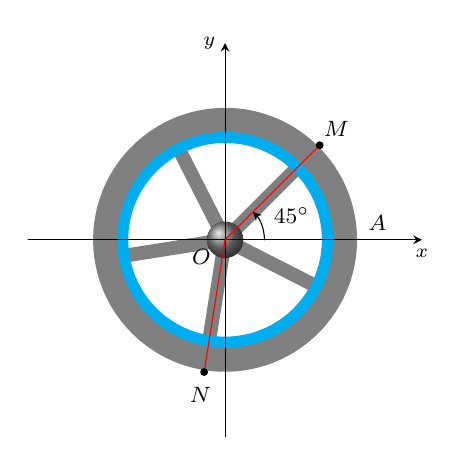
\begin{tikzpicture}[scale=1.0, font=\footnotesize,line join=round, line cap=round, >=stealth];		
			\draw[line width=5,color=gray] (0:0)--(45:1.3) ;
			\draw[line width=5,color=gray] (0:0)--(117:1.3) ;
			\draw[line width=5,color=gray] (0:0)--(189:1.3) ;
			\draw[line width=5,color=gray] (0:0)--(261:1.3) ;
			\draw[line width=5,color=gray] (0:0)--(333:1.3) ;
			\draw[line width=10,color=gray] (0:1.5) arc (0:360:1.5);
			\draw[line width=4,color=cyan] (0:1.3) arc (0:360:1.3);
			\fill[ball color=gray] (0:0) circle (.23);
			\draw[->] (-2.5,0) -- (2.5,0) node[below] {\scriptsize $x$};
			\draw[->] (0,-2.5) -- (0,2.5) node[left] {\scriptsize $y$};
			\draw (1.7,0) node[above right] {$A$};
			\draw (-0.3,0) node[below] {$O$};
			\draw  (45:2) node {$M$};
			\draw  (261:2) node {$N$};						
			\draw[color=red]  (0:0)--(45:1.7)  (0:0)--(261:1.7) ;
			\draw (20:0.9) node{$45^\circ$};		
			\draw[-stealth] (0:.5) arc (0:45:.5);		
			\draw[fill=black](45:1.7) circle (1.2pt) (261:1.7) circle (1.2pt);	
		\end{tikzpicture}
	}
	\loigiai{
		Ta có $\widehat{AON}=\left(\dfrac{360^\circ}{5} -45^\circ\right)+72^\circ=99^\circ$.\\
		Vậy $(Ox, ON)=-99^\circ+k360^\circ \; (k \in \mathbb{Z})$.
		
	}
	
\end{bt}

\begin{bt}%[Tex hóa SGK CD-CT,T7/22, TVN-099]%[1T1B1-6]
	\immini[thm]{Hải lí là một đơn vị chiều dài hàng hải, được tính bằng độ dài một cung chắn một góc $\alpha=\left(\dfrac{1}{60}\right)^{\circ}$ của đường kinh tuyến (Hình bên). Đổi số đo $\alpha$ sang radian và cho biết 1 hải lí bằng khoảng bao nhiêu kilômét, biết bán kính trung bình của Trái Đất là $6371\, km$. Làm tròn kết quả đến hàng phần trăm.}
	{{\begin{tikzpicture}[scale=1.2, font=\footnotesize,line join=round, line cap=round, >=stealth];
				\draw[fill=cyan!30 ] (0,0) circle (1.7);		
				\draw (-2,0) -- (2,0) ;
				\draw (0,-2)node[right] {\scriptsize $\text{Cực Nam}$} -- (0,2) node[right] {\scriptsize $\text{Cực Bắc}$};
				\path
				(0,0) coordinate (O)
				(48:1.7) coordinate (B)
				(55:1.7) coordinate (C);
				\draw  (0:0)--(48:1.7) (0:0)--(55:1.7);			
				\draw  (62:2) node[right,rotate=-43]{$\text{hải lí}$};
				\draw (0:1.7) arc (0:360:1.7);
				\draw (15:0.9) node{$\alpha=\left(\tfrac{1}{60}\right)^{\circ}$};		
				\draw (0.5,0) node[below] {Đường xích đạo};
				\pic["$ $"{shift={(1pt,3pt)}},draw,angle radius=6mm,angle eccentricity=1.79] {angle = B--O--C};	
	\end{tikzpicture}}}
	\loigiai{
		1 hải lí = $\alpha\cdot R=\dfrac{1\cdot \pi }{60\cdot 180}\cdot 6371 \approx 1{,}85$ km.
		
	}
	
\end{bt}
\cham{4}

\begin{bt}
	Chứng minh các hệ thức sau
	\begin{enumEX}{2}
		\item $\dfrac{1+\sin^4\alpha -\cos^4\alpha}{1-\sin^6\alpha -\cos^6\alpha}=\dfrac{2}{3\cos^2\alpha}$;
		\item $\dfrac{\sin^2\alpha (1+\cos \alpha )}{\cos^2\alpha \left(1+\sin \alpha \right)}=\dfrac{\sin \alpha +\tan \alpha}{\cos \alpha +\cot \alpha}$;
		\item $\dfrac{\tan \alpha -\tan \beta}{\cot \beta -\cot \alpha}=\tan \alpha \tan \beta $;
		\item $\dfrac{\cos^2\alpha -\sin^2\alpha}{\cot^2\alpha -\tan^2\alpha}=\sin^2\alpha \cos^2\alpha $.
		\item $\dfrac{1-4\sin^2x\cos^2x}{\left(\sin x+\cos x\right)^2}=\left(\sin x-\cos x\right)^2$;
		\item $\dfrac{\sin^2x-\cos^2x+\cos^4x}{\cos^2x-\sin^2x+\sin^4x}=\tan^4x$.
	\end{enumEX}
	\loigiai{
		\begin{enumerate}[a)]
			\item Ta có $\dfrac{1+\sin^4\alpha -\cos^4\alpha}{1-\sin^6\alpha -\cos^6\alpha}=\dfrac{1+(\sin^2\alpha +\cos^2\alpha )\left(\sin^2\alpha -\cos^2\alpha \right)}{1-\left[\left(\sin^2\alpha +\cos^2\alpha \right)^2-3\sin^2\alpha \cos^2\alpha \left(\sin^2\alpha +\cos^2\alpha \right)\right]}$ \\
			\phantom{Ta có $\dfrac{1+\sin^4\alpha -\cos^4\alpha}{1-\sin^6\alpha -\cos^6\alpha}$} $=\dfrac{1+\sin^2\alpha -\cos^2\alpha}{1-\left[1-3\sin^2\alpha \cos^2\alpha \right]}=\dfrac{2\sin^2\alpha}{3\sin^2\alpha \cos^2\alpha}=\dfrac{2}{3\cos^2\alpha}$.
			\item Ta có $\dfrac{\sin \alpha +\tan \alpha}{\cos \alpha +\cot \alpha}=\dfrac{\sin \alpha \left(1+\dfrac{1}{\cos \alpha}\right)}{\cos \alpha \left(1+\dfrac{1}{\sin \alpha}\right)}=\dfrac{\sin^2\alpha \left(1+\cos \alpha \right)}{\cos^2\alpha \left(1+\sin \alpha \right)}$.
			\item Ta có $\dfrac{\tan \alpha -\tan \beta}{\cot \beta -\cot \alpha}=\dfrac{\tan \alpha -\tan \beta}{\dfrac{1}{\tan \beta}-\dfrac{1}{\tan \alpha}}=\dfrac{\dfrac{\tan \alpha -\tan \beta}{\tan \alpha -\tan \beta}}{\tan \alpha \tan \beta}=\tan \alpha \tan \beta $.
			\item Ta có $\dfrac{\cos^2\alpha -\sin^2\alpha}{\cot^2\alpha -\tan^2\alpha}=\dfrac{\cos^2\alpha -\sin^2\alpha}{\dfrac{\cos^2\alpha}{\sin^2\alpha}-\dfrac{\sin^2\alpha}{\cos^2\alpha}}=\sin^2\alpha \cos^2\alpha \left(\dfrac{\cos^2\alpha -\sin^2\alpha}{\cos^4\alpha -\sin^4\alpha}\right)$ \\
			\phantom{Ta có $\dfrac{\cos^2\alpha -\sin^2\alpha}{\cot^2\alpha -\tan^2\alpha}$} $=\sin^2\alpha \cos^2\alpha \dfrac{1}{\cos^2\alpha +\sin^2\alpha}=\sin^2\alpha \cos^2\alpha $.
			\item Ta có $\dfrac{1-4\sin^2x\cos^2x}{\left(\sin x+\cos x\right)^2}=\dfrac{\left(\sin^2x+\cos^2x\right)^2-4\sin^2x\cos^2x}{\left(\sin x+\cos x\right)^2}$\\
			\phantom{Ta có $\dfrac{1-4\sin^2x\cos^2x}{\left(\sin x+\cos x\right)^2}$} $=\dfrac{\left(\sin^2x-\cos^2x\right)^2}{\left(\sin x+\cos x\right)^2}=\left(\sin x-\cos x\right)^2$.
			\item Ta có $\dfrac{\sin^2x-\cos^2x+\cos^4x}{\cos^2x-\sin^2x+\sin^4x}=\dfrac{\sin^2x-\cos^2x\left(1-\cos^2x\right)}{\cos^2x-\sin^2x\left(1-\sin^2x\right)}=\dfrac{\sin^2x\left(1-\cos^2x\right)}{\cos^2x\left(1-\sin^2x\right)}=\tan^4x$.
		\end{enumerate}
	}
\end{bt} \cham{35}

\begin{bt}
	Chứng minh các hệ thức sau không phụ thuộc vào $x$.
	\begin{enumEX}{2}
		\item $A=\dfrac{\sin^6x+\cos^6x+2}{\sin^4x+\cos^4x+1}$;
		\item $B=\dfrac{1+\cot x}{1-\cot x}-\dfrac{2+2\cot^2x}{\left(\tan x-1\right)\left(\cot^2x+1\right)}$.
	\end{enumEX}
	\loigiai{
		\begin{enumerate}[a)]
			\item Ta có $\sin^4\alpha +\cos^4\alpha =\left(\sin^2\alpha +\cos^2\alpha \right)^2-2\sin^2\alpha \cos^2\alpha =1-2\sin^2\alpha \cos^2\alpha $ \\
			\phantom{Ta có} $\sin^6\alpha +\cos^6\alpha =\left(\sin^2\alpha \right)^3+\left(\cos^2\alpha \right)^3$\\
			\phantom{Ta có $\sin^6\alpha +\cos^6\alpha$} $=\left(\sin^2\alpha +\cos^2\alpha \right)\left(\sin^4\alpha +\cos^4\alpha -\sin^2\alpha \cos^2\alpha \right)$ \\
			\phantom{Ta có $\sin^6\alpha +\cos^6\alpha$} $=\sin^4\alpha +\cos^4\alpha -\sin^2\alpha \cos^2\alpha =1-2\sin^2\alpha \cos^2\alpha -\sin^2\alpha \cos^2\alpha$\\
			\phantom{Ta có $\sin^6\alpha +\cos^6\alpha$} $=1-3\sin^2\alpha \cos^2\alpha $.\\
			Do đó $A=\dfrac{1-3\sin^2\alpha \cos^2\alpha +2}{1-2\sin^2\alpha \cos^2\alpha +1}=\dfrac{3\left(1-\sin^2\alpha \cos^2\alpha \right)}{2\left(1-\sin^2\alpha \cos^2\alpha \right)}=\dfrac{3}{2}$.\\
			Vậy $A$ không phụ thuộc vào $x$.
			\item Ta có $B=\dfrac{1+\dfrac{1}{\tan x}}{1-\dfrac{1}{\tan x}}-\dfrac{2+\dfrac{2\cos^2x}{\sin^2x}}{\left(\tan x-1\right)\dfrac{1}{\sin^2x}}=\dfrac{\tan x+1}{\tan x-1}-\dfrac{2\left(\sin^2x+\cos^2x\right)}{\tan x-1}$\\
			\phantom{Ta có $B$} $=\dfrac{\tan x+1-2}{\tan x-1}=1$.\\
			Vậy $B$ không phụ thuộc vào $x$.
		\end{enumerate}
	}
\end{bt} \cham{20}
